\chapter{Cases}\label{ch:cases}

A case is one run: one template, one mesh and one flight condition. Make it with
\file{newCase.sh} and run it with \file{Allrun}. \file{runCase.sh} does the two
steps for each line of a sweep file (\cref{ch:sweeps}).

\section{Make a case}\label{sec:make-case}

\subsection{Command}

\begin{shell}
./newCase.sh <run-dir> --mesh <mesh-dir> [options]
\end{shell}

\begin{longtable}{@{}P{0.32\linewidth} P{0.62\linewidth}@{}}
\caption{Options of \texttt{newCase.sh}.}\label{tab:newcase}\\
\toprule
Option & Function \\
\midrule
\endfirsthead
\toprule
Option & Function \\
\midrule
\endhead
\ent{--mesh <mesh-dir>} & Mandatory. The path of a mesh that \file{Allmesh} made. \\
\ent{--Minf <M>} & Free-stream Mach number. \\
\ent{--pInf <Pa>}, \ent{--Tinf <K>} & Free-stream static pressure and temperature. \\
\ent{--alpha <deg>}, \ent{--beta <deg>} & Angle of attack and angle of sideslip. \\
\ent{--Ti <->}, \ent{--nuRatio <->} & Free-stream turbulence intensity and ratio $\nu_t/\nu$. \\
\ent{--np <N>} & Number of subdomains in \file{system/decomposeParDict}. \\
\ent{--socket <S>} & Binds the run to socket \val{S}, one process per physical core (\cref{sec:binding}). \val{none} disables the binding. \\
\ent{--refine tip}, \ent{--refine fins} & Runs \file{Allrefine} on the new case (\cref{sec:refine}). \\
\ent{--init <run-dir>} & Starts from the latest time of another run (\cref{sec:init}). \\
\ent{--solver central}, \ent{--solver pimple} & Template \file{case-central/} (default) or \file{case-pimple/}. \\
\bottomrule
\end{longtable}

The flow options change entries in \file{system/flowConditions}. The options that you
do not give keep the values of the template (\cref{tab:flowconditions}).

\begin{note}
For \file{newCase.sh}, \ent{--mesh} and \ent{--init} are paths. Only
\file{runCase.sh} accepts a name without a path.
\end{note}

\subsection{Steps that newCase.sh does}

\begin{figure}[htbp]
  \centering
  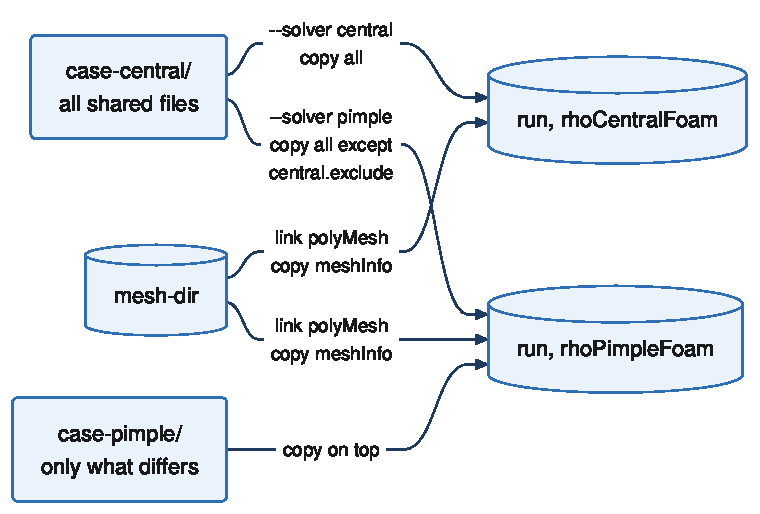
\includegraphics[width=0.75\linewidth]{figures/pdf/templates.pdf}
  \caption{How \texttt{newCase.sh} assembles a case from the templates and a mesh.}
  \label{fig:templates}
\end{figure}

\begin{steps}
\item It stops if \ent{--mesh} is missing, if the mesh has no
  \file{constant/polyMesh}, or if \file{<run-dir>} exists.
\item It copies \file{case-central/} into \file{<run-dir>}, without the mesh, the logs,
  \file{0/}, \file{processor*}, \file{postProcessing/} and the time directories. With
  \ent{--solver pimple}, it leaves out the files in \file{case-pimple/central.exclude}
  and then copies \file{case-pimple/} on top (\cref{fig:templates}).
\item It links \file{constant/polyMesh} to the mesh. With \ent{--refine} it copies it.
\item It copies \file{<mesh-dir>/meshInfo} to \file{constant/meshInfo}.
\item It copies \file{common/Allrun}, \file{common/Allrefine} and
  \file{common/machineLog.py} into the case.
\item It writes \file{run.info} with the case name, the date, the commit of the
  repository, the mesh, the number of cells and the options.
\item It renders each \file{*.j2} file with the values in \file{config.json}
  (\cref{sec:config-json}), and removes the \file{*.j2} file.
\item It writes each flow option into \file{system/flowConditions}. It stops if the
  entry does not exist.
\item It writes \ent{--np} into \file{decomposeParDict} and \ent{--socket} into the
  file \file{socket}. With \ent{--init}, it writes the path of the other run into
  \file{initFrom} and into \file{run.info}.
\item With \ent{--refine}, it runs \file{Allrefine}.
\item It adds to \file{run.info} the fingerprint of the mesh (\ent{meshHash}) and the
  physical definition of the case (block \ent{flow}, \cref{sec:nektar-same}).
\end{steps}

\section{Run a case}\label{sec:run-case}

\subsection{Command}

\begin{shell}
cd <run-dir>
./Allrun        # parallel, numberOfSubdomains from system/decomposeParDict
./Allrun 8      # parallel on 8 processes; writes 8 into decomposeParDict
./Allrun 1      # serial
\end{shell}

\subsection{Steps that Allrun does}

\Cref{fig:allrun} shows the steps.

\begin{figure}[htbp]
  \centering
  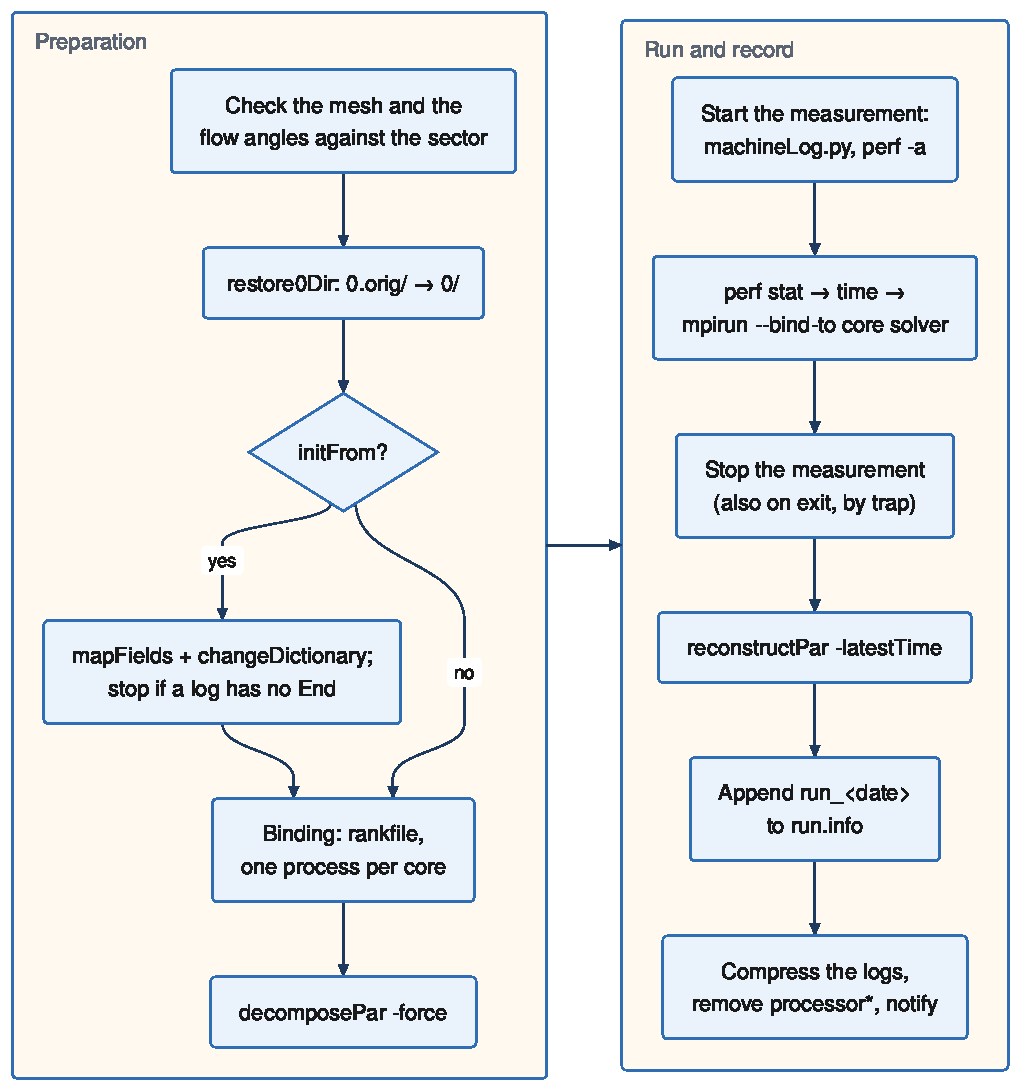
\includegraphics[width=0.9\linewidth]{figures/pdf/allrun.pdf}
  \caption{Steps of \texttt{Allrun}.}
  \label{fig:allrun}
\end{figure}

\begin{steps}
\item It stops if \file{constant/polyMesh} does not exist.
\item It compares \ent{alpha} and \ent{beta} in \file{flowConditions} with
  \ent{sector} in \file{meshInfo} (\cref{tab:sectors}). It stops if the mesh cannot
  show the flow angle.
\item It copies \file{0.orig/} to \file{0/}. If \file{initFrom} exists, it maps the
  other run onto \file{0/} (\cref{sec:init}).
\item It sets the binding of the processes (\cref{sec:binding}).
\item It runs \cmd{decomposePar -force}.
\item It starts the measurement (\cref{sec:measurement}) and runs the solver with
  \cmd{mpirun}. It stops the measurement when the solver ends. A trap also stops it
  if \file{Allrun} stops early.
\item It runs \cmd{reconstructPar -latestTime}, and removes \file{processor*} if that
  step ends correctly.
\item It adds a record \ent{run_<date>} to \file{run.info} (\cref{sec:runinfo}),
  compresses the logs with \cmd{xz} and sends the notification (\cref{sec:notify}).
\end{steps}

\begin{table}[htbp]
\centering
\caption{Flow angles that each mesh sector permits.}\label{tab:sectors}
\begin{tabular}{@{}ll@{}}
\toprule
\ent{sector} & Permitted angles \\
\midrule
\val{quarter} & $\alpha = 0$ and $\beta = 0$ \\
\val{half} & $\beta = 0$ (the default mesh) \\
\val{full} & All angles \\
\bottomrule
\end{tabular}
\end{table}

\subsection{Process binding}\label{sec:binding}

\file{Allrun} binds each MPI process to one physical core when:
\begin{itemize}
\item the case has a file \file{socket} with a socket number, or
\item the computer has one socket and the number of processes is not more than the
  number of physical cores.
\end{itemize}

It writes a \file{rankfile} with process $i$ on core $i$ of the socket, and runs
\cmd{mpirun --bind-to core}. It stops if the processes are more than the cores of the
socket. To run without binding, for example a short test beside a sweep, write
\val{none} in the file \file{socket}.

\begin{caution}
\file{Allrun} does not use the OpenFOAM function \cmd{runParallel}, because it always
adds \cmd{--oversubscribe}. With that option, Open MPI 5 ignores the
\file{rankfile}, and each process can move to all CPUs. \file{run.info} then shows a
binding that did not occur. To check the binding of a run, examine each process:
\cmd{taskset -cp <pid>} must give the two threads of one core.
\end{caution}

\subsection{End of a run}

The run stops at \ent{endTime}, or when the stop criterion finds that the mean of
$C_D$ is constant (\cref{sec:stop-criterion}). The record in \file{run.info} gives
\ent{status ok} if the solver log ends with \val{End}.

\subsection{Continue a run}

\file{controlDict} has \ent{startFrom latestTime}. Run \cmd{./Allrun} again in the same
directory to continue from the last time directory. The continuation adds a new
record to \file{run.info} and writes the function objects into a new directory with
its start time.

\begin{caution}
\file{Allrun} runs \cmd{decomposePar -force}, which removes the \file{processor*}
directories. If the solver stopped before \cmd{reconstructPar}, run
\cmd{reconstructPar -latestTime} before you run \cmd{./Allrun} again. If you do not,
you lose the data after the last reconstructed time.
\end{caution}

On the first continuation, read the start time in the solver log. Make sure that it
is the last time and not 0.

\subsection{Start a run again from zero}

\begin{steps}
\item Remove the time directories and the processor directories:
  \cmd{rm -rf [1-9]* processor*}.
\item Run \cmd{./Allrun}.
\end{steps}

\file{./Allclean} also removes \file{constant/polyMesh}. After \file{./Allclean}, make a
new case with \file{newCase.sh}.

\section{Start from another run}\label{sec:init}

\cmd{newCase.sh --init <run-dir>} starts the case from the solution of another run
instead of the uniform free stream. The sweep uses it from a coarse mesh to the next
finer mesh at the same flight condition, as the OpenFOAM ToolChain does
\citep[§5.4]{toolchain2026}. The fine mesh starts with the shock, the wake and the
boundary layer in place. The two runs can use different solvers. After
\cmd{restore0Dir}, \file{Allrun} does these steps:

\begin{steps}
\item It reads the value of each \val{fixedValue} patch in \file{0/}. These are the
  values of this run: in a supersonic case, \ent{p} on \val{inlet}.
\item It runs \cmd{mapFields <run-dir> -consistent -sourceTime latestTime}. This maps
  the internal field and the patch values. The other run can have another mesh of
  the same domain and patches.
\item It runs \cmd{changeDictionary} to write back the values of step 1.
\item It stops if the log of \cmd{mapFields} or of \cmd{changeDictionary} does not end
  with \val{End}.
\end{steps}

The free-stream entries of the patches (\ent{freestreamValue}, \ent{inletValue},
\ent{fieldInf}) are not mapped. They keep the values of this run. The other run must
have a time directory with the solution.

\begin{caution}
\cmd{mapFields} stops with a segmentation fault when it maps onto the same mesh
($h0 \to h0$), at the field \ent{Ma} (2026-10-17). The supersonic chain does this
mapping (pimple $\to$ central on $h0$). \file{Allrun} now stops the run. Before this
check, the run continued from the uniform free stream and \file{Allrun} reported the
mapping as correct. See \cref{sec:ts-mapfields}.
\end{caution}

\section{Refine the mesh near the fins (optional)}\label{sec:refine}

\begin{shell}
./Allrefine          # same as ./Allrefine tip
./Allrefine tip      # cell set finTip: a band around the fin tip
./Allrefine fins     # cell set finBox: the full fin, from root to tip
\end{shell}

Do this procedure in the case directory, before \cmd{./Allrun}, or give
\ent{--refine} to \file{newCase.sh}. \file{Allrefine} does these steps:

\begin{steps}
\item It stops if \file{0/U} exists. \cmd{refineMesh} maps the fields, so a refinement
  after a run changes the results.
\item It stops if \file{meshInfo} does not have \ent{fins true} and \ent{finTipR}.
\item It replaces the link to the mesh with a copy, so that it does not change the
  shared mesh.
\item It runs \cmd{topoSet}. \file{system/topoSetDict} makes the cell sets from the fin
  geometry in \file{meshInfo}.
\item It runs \cmd{refineMesh}. Each cell in the set becomes 8 cells.
\item It runs \cmd{checkMesh} and \cmd{renumberMesh}, and writes the new number of
  cells into \file{meshInfo}.
\end{steps}

\begin{tabularx}{\linewidth}{@{}l P{0.34\linewidth} L@{}}
\toprule
Set & Region & Effect on \yplus \\
\midrule
\val{finTip} & Annulus from $\texttt{finTipR} - \texttt{tipBand}$ to $\texttt{finTipR} + \texttt{margin}$ & None. The region does not touch the body. \\
\val{finBox} & Cylinder of radius $\texttt{finTipR} + \texttt{margin}$ & The first body cell below the fins is half as thick, so \yplus{} there is approximately half. \\
\bottomrule
\end{tabularx}
